\documentclass[letterpaper,10pt,titlepage,fleqn]{article}

%example of setting the fleqn parameter to the article class -- the below sets the offset from flush left (fl)
\setlength{\mathindent}{1cm}

\usepackage{graphicx}                                        

\usepackage{amssymb}                                         
\usepackage{amsmath}                                         
\usepackage{amsthm}                                          

\usepackage{alltt}                                           
\usepackage{float}
\usepackage{color}

\usepackage{url}

\usepackage{balance}
\usepackage[TABBOTCAP, tight]{subfigure}
\usepackage{enumitem}

\usepackage{pstricks, pst-node}

%the following sets the geometry of the page
\usepackage{geometry}
\geometry{textheight=9in, textwidth=6.5in}

% random comment

\newcommand{\cred}[1]{{\color{red}#1}}
\newcommand{\cblue}[1]{{\color{blue}#1}}

\usepackage{hyperref}

\usepackage{textcomp}
\usepackage{listings}

\def\name{D. Kevin McGrath}

%% The following metadata will show up in the PDF properties
\hypersetup{
  colorlinks = true,
  urlcolor = black,
  pdfauthor = {\name},
  pdfkeywords = {cs311 ``operating systems'' files filesystem I/O},
  pdftitle = {CS 311 Project},
  pdfsubject = {CS 311 Project},
  pdfpagemode = UseNone
}

\parindent = 0.0 in
\parskip = 0.2 in

\begin{document}

%to remove page numbers, set the page style to empty

\section*{Surface Integral}
\hrule

La di da...

this is a new paragraph

and another one

and yet a third...or is it fourth?

In physics (and everywhere else), 
\begin{eqnarray}
  x =& \frac{-b \pm \sqrt{b^2 - 4ac}}{2a}\\
  x =& \frac{-b \mp \sqrt{b^2}}{2a}
\end{eqnarray}.

\centerline{\includegraphics[width=0.5\textwidth]{maxwell.eps}}

%in order to use enumerated lists, you would use the itemize environment
\begin{itemize}
\item This is the first bullet
\item[\&] If I want to change the bullet, I use the syntax 
	``$\backslash$item[new\_bullet]''
\end{itemize}

Enumerate is identical to itemize in all options and syntax, but the name of 
the environment is enumerate, rather than itemize.

$\nabla$ is created via the use of $\backslash$nabla. Which is the proper 
name for the del operator, as it turns out.

To create greek letters, just use $\backslash$name, replacing name with the 
character you want (case matters!). Beware $\backslash$epsilon ($\epsilon$) vs 
$\backslash$varepsilon$\varepsilon$.

For the rest of the symbols, see the resources linked from the assignment.

\end{document}
